\chapter{Kwaliteitsbewaking}
In dit hoofdstuk wordt beschreven hoe de kwaliteit van het product gewaarborgd wordt.
Dit hoofdstuk is onderverdeeld in: proces, ontwerpen, testing en documentatie.
\section{Proces}
De ontwerp en realisatie fases van het project worden ondersteund door middel van de scrum methodiek.
\whitespace
Tijdens de realisatieperiode worden alle fases van de SDLC (figuur \ref{fig:SLDC}) te doorlopen.
Hierbij wordt de requirement analysis uitgevoerd aan de hand van het onderzoek.
Daarna worden er 2 weken geplant voor het designen van het systeem.
Vervolgens worden er 9 sprints geplant voor het implementeren en testen van het systeem. \\
% \todo[inline]{is 1 sprint te weinig en zijn 2 sprints te veel}
\begin{graphic}
    \captionsetup{type=figure}
    \caption{Software Development Life Cycle (SDLC)}
    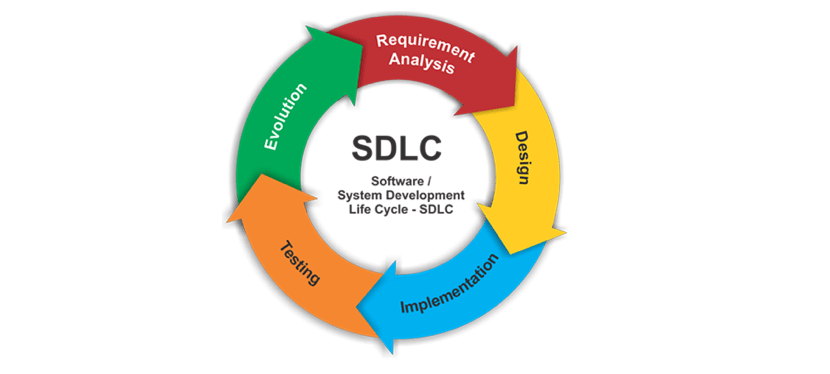
\includegraphics[scale=0.4]{SDLC}
    \label{fig:SLDC}
\end{graphic}
\textbf{Requirement analysis:} Door middel van de requirement analyse (het onderzoek) worden de requirements opgesteld.
Tijdens de sprint planning worden de requirements verwerkt tot behapbare user stories, zodat ze tijdens de sprints gemaakt kunnen worden. \\
\textbf{Design:} De eisen en wensen die vanuit de requirement analyse worden gebruikt om het ontwerp te maken.
Hoe er ontwerpt wordt is toegelicht in hoofdstuk \ref{sec:Ontwerpen}.\\
\textbf{Inplementation:}
De eisen en wensen worden geïmplementeerd volgens het ontwerp binnen het systeem.\\
\textbf{Testing:} Door de loop van het realisatieproces worden de verschillende testen van het V-Model uitgevoerd, zie hoofdstuk \ref{sec:Testing} voor meer informatie.\\
\textbf{Evolution:} Er wordt met regelmaat feedback momenten gehouden waar het product gedemonstreerd wordt aan de bedrijfsbegeleider.
Dit wordt gedaan om de projectvoortgang te bewaken op basis van de gemaakte eisen en wensen.
\subsection{Code reviews}
Tijdens de realisatiefase worden er meerdere code reviews gehouden om de codekwaliteit te waarborgen.
Deze code reviews worden gehouden met de backend en frontend developers van Snakeware.
De code zal ook beoordeeld worden op coderingsstandaarden maar ook structuur.
\subsection{Versiebeheer}
Binnen Snakeware wordt er gebruikgemaakt van Bitbucket en git voor het versiebeheer van de code, dit zal ook gebruikt worden voor de afstudeeropdracht.
Verder zal er ook gebruikgemaakt worden van een CI-pipeline die wordt opgezet om de code automatisch te testen.
\section{Ontwerpen}
\label{sec:Ontwerpen}
Tijdens het ontwerpen wordt er gebruikgemaakt van UML.
Er zullen verschillende UML diagrammen gemaakt worden op basis van het 4 + 1 model.
Dit wordt gerealiseerd na het onderzoek wanneer de requirements bekend zijn.
In figuur \ref{fig:4+1Model} wordt beschreven welke diagrammen mogelijk gebruikt kunnen worden voor de verschillende views van het 4 + 1 model.
\begin{graphic}
    \captionsetup{type=figure}
    \caption{Verschillende UML diagrammen die mogelijk gebruikt kunnen worden bij de verschillende views \Parencite{4p1ModelViews}}
    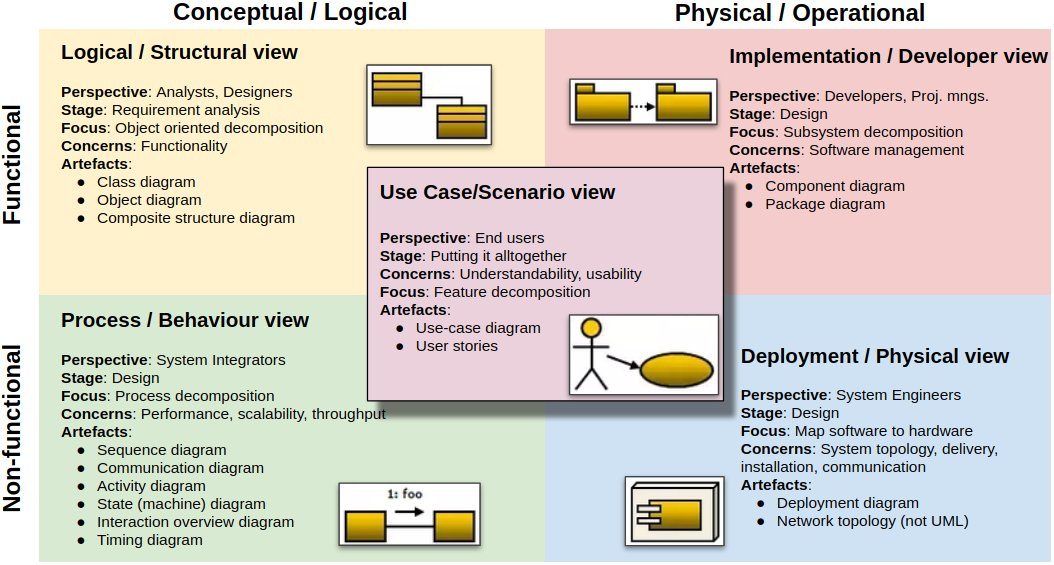
\includegraphics[scale=0.4]{4p1ModelViews}
    \label{fig:4+1Model}
\end{graphic}
\section{Testing}
\label{sec:Testing}
Tijdens de realisatieperiode wordt er gebruikgemaakt van de V-Model.
Het V-Model \ref{fig:VModel} toont dat er voor de verschillende design lagen van het systeem verschillende testen gebruikt worden.
De verschillende units/modules van code worden getest door middel van unit testing.
Vervolgens worden de samen hangende units/modules getest door integratie testen om het softwaredesign te kunnen valideren.
De laag boven softwaredesign is systeemanalyse, dit wordt getest door middel van systeem testing.
Daarna worden de requirements gevalideerd door acceptatie testen uit te voeren met de stakeholders.
\begin{graphic}
    \captionsetup{type=figure}
    \caption{V-Model \Parencite{VModel}}
    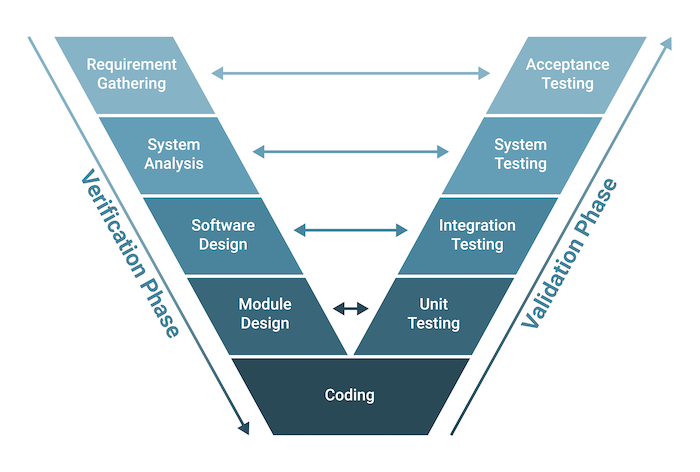
\includegraphics[scale=0.4]{VModel}
    \label{fig:VModel}
\end{graphic}
\section{Documentatie}
De kwaliteit van de documentatie wordt gevalideerd door de bedrijfsbegeleider, docentbegeleider en medestudenten.
Er wordt met de docent en bedrijfsbegeleider een keer per week afgesproken om de kwaliteit en de voortgang van de verschillende zaken van de afstudeerperiode te bespreken, waaronder de verslaglegging.
Verder zal er per hoofdstuk feedback worden gevraagd om de kwaliteit van de documentatie hoog te houden.
In de verslagen zullen onderbouwd door bronnen en deze zullen gedocumenteerd worden door APA 7 richtlijnen.
Voor het indienen van een document is het vereist dat minimaal een conceptversie is beoordeeld door zowel de bedrijfsbegeleider als de docentbegeleider.
